Gaia travels among planets via (bidirectional) wormholes. She starts from planet $X$ and plans to reach planet $Y$. There may or may not exist a wormhole that connects planets $X$ and $Y$ directly. Therefore, on some occasions, it is necessary to traverse along a sequence of wormholes rather than just a single one. Some intermediate planets other than $X$ and $Y$ are visited while transferring from one wormhole to another. Given the temperature of all planets, Gaia would like to search for a sequence of wormholes from planet $X$ to $Y$ that minimizes the temperature difference between the hottest visited planets and the coldest visited one. For the sake of simplicity, we assume that planet $X$ has temperature $X$ (K) for each $X$. 

\begin{figure}[!h]
\centering
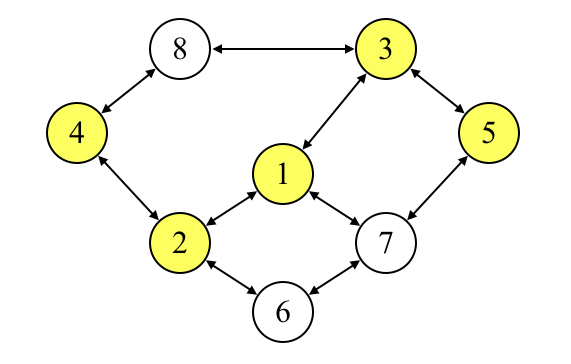
\includegraphics[width=0.6\textwidth]{image/D-fig1.png}
\caption{If $X = 4$ and $Y = 5$, then the best route for Gaia to reach $Y$ from $X$ is $4 \rightarrow 2 \rightarrow 1 \rightarrow 3 \rightarrow 5$ because it has the smallest temperature difference $4$. \label{fig:drawing}}
\end{figure}
